\documentclass{fkssolpub}

\usepackage[czech]{babel}
\usepackage{fontspec}
\usepackage{fkssugar}
\usepackage{amsmath}
\usepackage{graphicx}
\usepackage{listings}
\usepackage{color}

\definecolor{codegray}{rgb}{0.5,0.5,0.5}
\lstset{
  basicstyle=\ttfamily,
  breaklines=true,
  keywordstyle=\color{blue},
  numberstyle=\color{codegray}\ttfamily,
  numbers=left,
  }

\author{Ondřej Sedláček}
\school{Gymnázium Oty Pavla} 
\series{4}
\problem{3} 

\begin{document} 

\section{Problém 2}

Abychom do automatu pro ovládání dveří výtahu zahrnuli i senzor překážky,
stačí přidat jen jediný přechod do Obrázku 11 z časopisu:

\begin{figure}[h!]
  \centering
  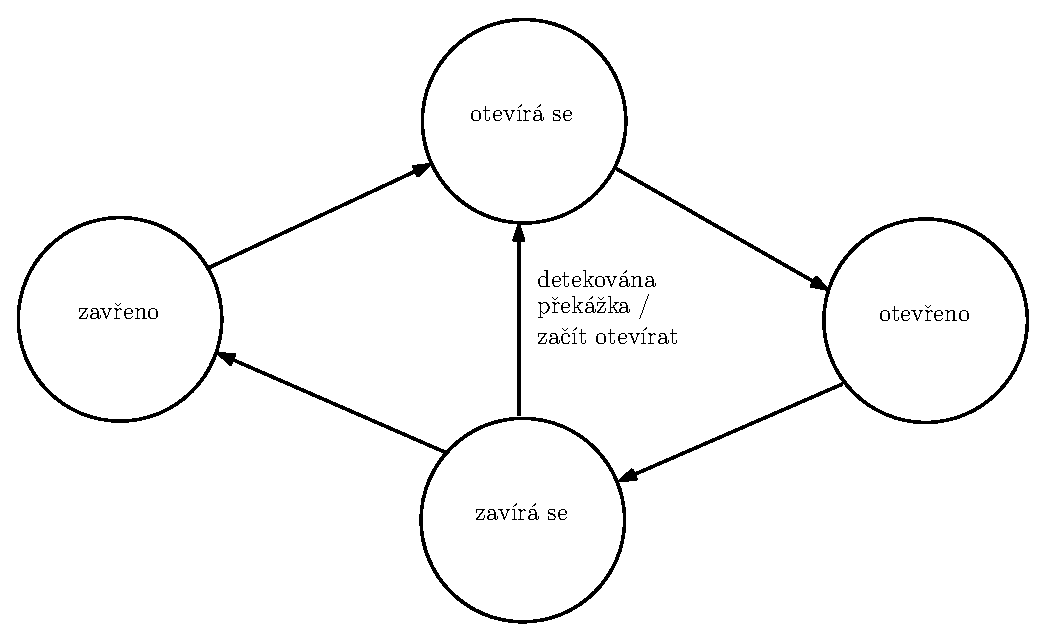
\includegraphics{Automat dveří.eps}
  \caption{Automat dveří}
  \label{fig:automata}
\end{figure}

Teď se musíme zamyslet nad tím, jak ten stroj pozná, že se před ním nachází
překážka. Záleží též na tom, kde je ten senzor umístěn. Zde budu předpokládat,
že se senzor nachází na těch pohybující se částí dveří tak, že budou schopny
změřit díru mezi oběmi částmi dveří. Tím pádem pokud senzor bude vracet
hodnoty od 0 do 1, pak by v případě, kdy překážka nebrání v zavírání,
budou hodnoty otevřenosti dveří a hodnoty senzoru stejné (samozřejmě
v rozmezí odchylky). Proto pro detekci překážky musí platit:

\[
  |\text{senzor} - \text{dveře}| > \text{odchylka}
\]

Protože jsme v automatu přidali jen jeden přechod, pro implementaci v kódu
6 z časopisu nám stačí tento kód jen mírně upravit (předpokládám, že v simulátoru
je implementována metoda \lstinline{e.getDoorSensor(id: str, floor: int) -> float}):


\begin{lstlisting}[language=Python]

# ...

def jeZdePrekazka(e: elevators.Simulator, id: str, floor: int) -> bool:
    return abs(
        e.getDoorSensor(id, floor) - e.getDoorsPosition(id, floor)
    ) > GD.PRECISION

def prechodovaFunkce(e: elevators.Simulator) -> None:
    # ...

    # dole se zavirajicimi se dvermi
    elif GD.posState == GD.POS_DOWN and GD.doorState == 2:
        if jeZdePrekazka(e, 'A', GD.POS_DOWN):
            GD.doorState = 1
        elif zavirejDvere(e, ’A’, GD.POS_DOWN):
            GD.doorState = 0
            GD.posState = 11
            e.speedUp(’A’)
    # nahore se zavirajicimi se dvermi
    elif GD.posState == GD.POS_UP and GD.doorState == 2:
        if jeZdePrekazka(e, 'A', GD.POS_UP):
            GD.doorState = 1
        elif zavirejDvere(e, ’A’, GD.POS_UP):
            GD.doorState = 0
            GD.posState = 12
            e.speedDown(’A’)

    # ...

\end{lstlisting}

\end{document}
